\section{Post-Quantum Provenance Protocol}
\label{sec:method}

\begin{figure*}[!t]
\centering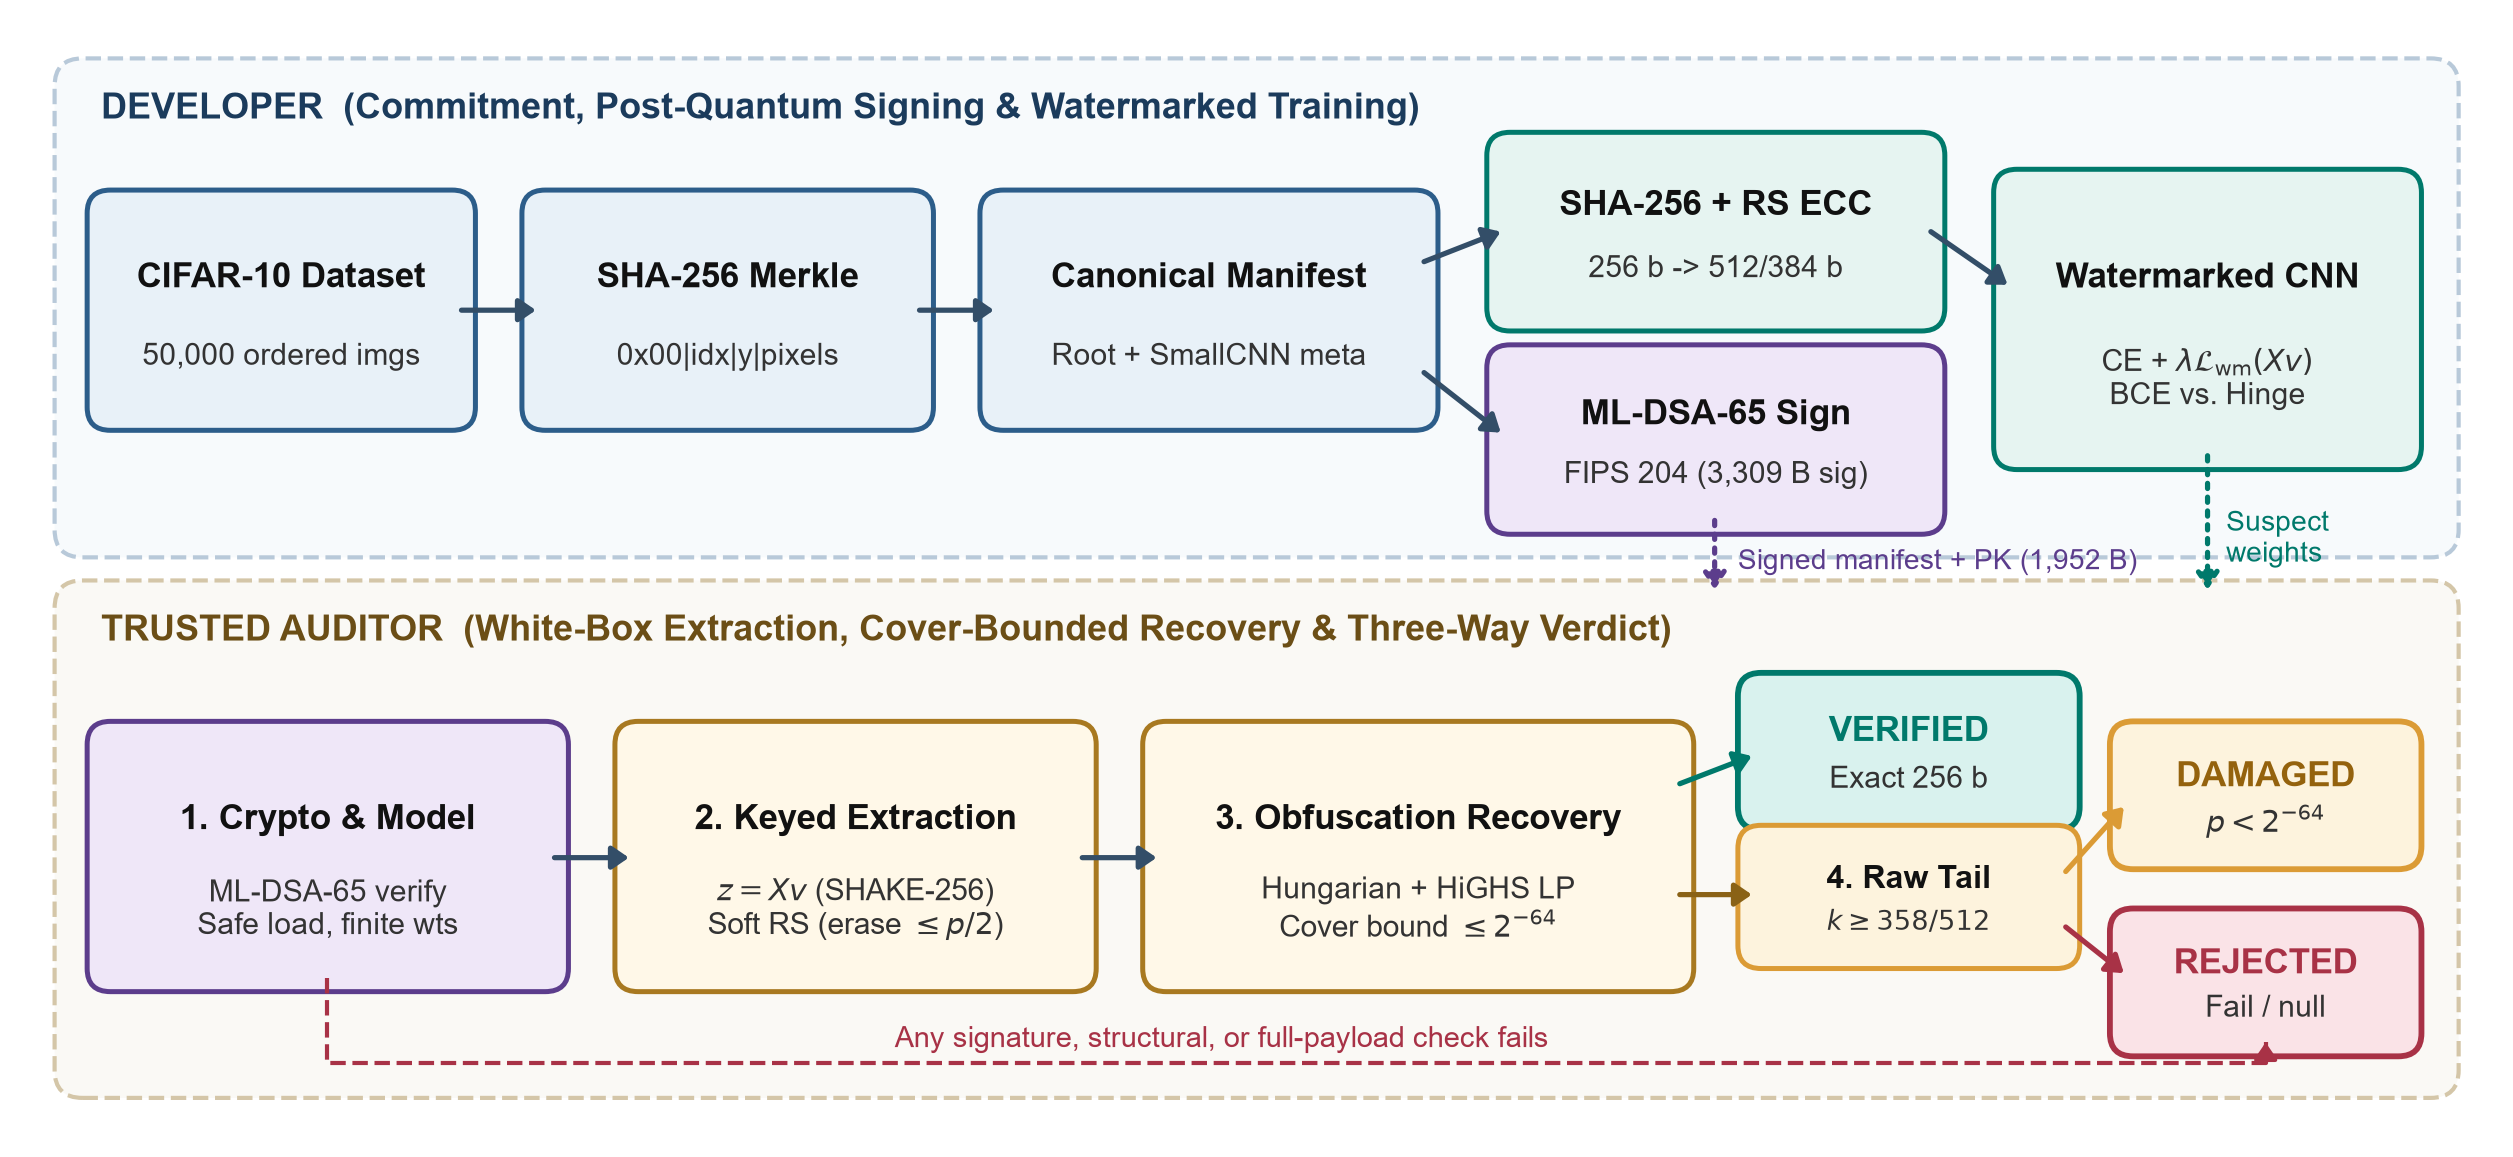
\includegraphics[width=0.96\textwidth]{figures/00_architecture.png}
\caption{End-to-end post-quantum provenance protocol. Top: the developer commits to the ordered CIFAR-10 training set via a SHA-256 Merkle tree, signs a canonical manifest with ML-DSA-65, and embeds its Reed--Solomon-encoded 256-bit digest into \textsc{SmallCNN} via a keyed projection. Bottom: the white-box auditor verifies the signature and tensor integrity, decodes the watermark with soft erasures, applies Cover-bounded alignment when needed, and issues \textsc{Verified}, \textsc{Damaged}, or \textsc{Rejected}.}\label{fig:arch}
\end{figure*}

\subsection{Actors, Threat Model, and Scope}
Our protocol (Fig.~\ref{fig:arch}) involves two parties: a \textbf{Developer}, who commits to a training dataset, signs a release manifest, and trains a watermarked classifier; and a \textbf{Trusted Auditor}, who holds white-box access to a suspect model checkpoint alongside the developer's public key, signed manifest, and secret watermark key~\cite{projectResults}. We model three adversaries:
\begin{enumerate}
  \item \textbf{Remover:} Possesses the model weights and applies post-training modifications---Gaussian noise, magnitude pruning, quantization, fine-tuning, function-preserving channel permutation or scaling, or same-layer watermark overwriting---to erase provenance while keeping classification accuracy within 5 percentage points of the clean watermarked model.
  \item \textbf{Forger:} Attempts to pass off an unmarked or third-party model as the developer's release by altering manifest fields, forging signatures, or exploiting weak verification rules (such as checking only a short prefix of the payload).
  \item \textbf{Poisoner:} Modifies, re-labels, or reorders training samples after the dataset commitment has been signed.
\end{enumerate}

To keep all claims defensible, we state four explicit boundaries: (i)~verification is white-box and assumes a trusted auditor who protects the secret watermark key; (ii)~the dataset Merkle root proves \emph{which} dataset was committed at signing time, not that samples were clean beforehand or that the weights were trained exclusively on those samples; (iii)~model distillation (training a new model from API outputs) is out of scope; and (iv)~manifest timestamps are self-declared, so ownership priority disputes require an external timestamping authority (e.g., RFC~3161) or transparency log.

\subsection{Dataset Commitment and ML-DSA-65 Manifest Signing}
To bind all 50,000 ordered CIFAR-10 training images~\cite{cifar10} into a compact commitment, the developer constructs a domain-separated SHA-256 Merkle tree~\cite{merkle1987digital}. Each leaf hashes a domain tag, sample index, label, and raw uint8 pixel bytes:
\begin{equation}
  h_i = \mathrm{SHA256}\bigl(\texttt{0x00} \parallel \mathrm{u64be}(i) \parallel \mathrm{u16be}(y_i) \parallel \mathbf{x}_i\bigr),
\end{equation}
while internal nodes hash $\texttt{0x01} \parallel h_{\mathrm{left}} \parallel h_{\mathrm{right}}$ (promoting odd nodes unchanged). Domain separation prevents second-preimage confusion between leaves and internal nodes, and embedding the index $i$ prevents silent sample reordering.

The resulting 32-byte root is placed in a canonical JSON manifest (sorted keys, no extraneous whitespace) containing the developer identifier, public-key identifier ($\mathrm{SHA256}(pk)_{[0:16]}$), architecture (\textsc{SmallCNN}, width 32, 160,234 parameters), watermark payload bit length (256), and UTC timestamp. The developer signs the exact canonical manifest bytes $M$ using \textbf{ML-DSA-65} (NIST FIPS~204~\cite{nist204}), producing a 3,309-byte signature verifiable under a 1,952-byte public key. Because embedding 26,472 signature bits directly inside a 160k-parameter network is impractical, the signed manifest ships beside the release while the watermark payload is defined as the full 256-bit digest
\begin{equation}
  p = \mathrm{SHA256}(M) \in \{0,1\}^{256}.
\end{equation}
Excluding $p$ from $M$ avoids circularity, while ensuring that altering any manifest field flips roughly half of the embedded payload bits.

\subsection{Error-Corrected Projection Watermarking}
Before training, the 32-byte payload $p$ is encoded with a systematic Reed--Solomon (RS) code over $\mathrm{GF}(256)$~\cite{reed1960polynomial}: \textbf{RS32} appends 32 parity bytes to yield $n=512$ binary codeword bits (correcting $e$ byte errors and $f$ erasures whenever $2e+f \le 32$), whereas \textbf{RS16} appends 16 parity bytes to yield $n=384$ bits ($2e+f \le 16$).

Following Uchida \emph{et al.}~\cite{uchida2017embedding}, we select the final convolutional layer (\texttt{features.6.0.weight}, shape $128 \times 64 \times 3 \times 3$) and average across its 128 output filters to obtain a 576-element carrier vector $v \in \mathbb{R}^{576}$ ($C=64$ input channels $\times K=9$ spatial taps). Output-channel averaging makes the carrier intrinsically invariant to permuting the carrier's output filters. A 32-byte secret watermark key is expanded deterministically with SHAKE-256 into a projection matrix $X \in \{-1,+1\}^{n \times 576}$, producing raw projection logits $z = Xv \in \mathbb{R}^n$.

Let $s_i = 2b_i - 1 \in \{-1,+1\}$ denote the signed target for codeword bit $b_i \in \{0,1\}$. The model is trained jointly with classification cross-entropy $\mathcal{L}_{\mathrm{CE}}$ and a weighted watermark objective $\mathcal{L}_{\mathrm{total}} = \mathcal{L}_{\mathrm{CE}} + \lambda \mathcal{L}_{\mathrm{wm}}$ comparing two formulations:
\begin{align}
  \mathcal{L}_{\mathrm{BCE}} &= \frac{1}{n}\sum_{i=1}^{n} \log\!\bigl(1 + \exp(-s_i z_i)\bigr), \label{eq:bce}\\
  \mathcal{L}_{\mathrm{hinge}} &= \frac{1}{n}\sum_{i=1}^{n} \max\bigl(0,\, m - s_i z_i\bigr). \label{eq:hinge}
\end{align}
Both penalize sign errors, but their gradients diverge sharply once a bit is correctly embedded. Because $\mathcal{L}_{\mathrm{BCE}}$ never vanishes, SGD continues enlarging the shared mean filter $v$ until weight decay counterbalances it, crowding out per-filter discriminative features. In contrast, $\mathcal{L}_{\mathrm{hinge}}$ contributes zero loss and zero gradient once $s_i z_i \ge m$, preserving classification capacity at the expense of leaving individual projection scores close to the boundary $m$.

\subsection{White-Box Verification, Obfuscation Recovery, and Verdicts}
Given a suspect checkpoint, release manifest, trusted public key, and watermark key, the auditor runs a strict staged pipeline~\cite{projectResults}:
\begin{enumerate}
  \item \textbf{Cryptographic and structural checks:} Verify the ML-DSA-65 signature on $M$, verify key-ID consistency, load checkpoint tensors safely without Python unpickling (rejecting crafted pickle payloads), check exact parameter count at signed width 32, reject any \texttt{NaN}/\texttt{Inf} weights, and enforce full 256-bit payload verification (preventing short-prefix forgery).
  \item \textbf{Soft-erasure RS decoding:} Compute $z = Xv$, map signs $\mathbb{I}[z_i > 0]$ to received bytes, and assign each byte a confidence equal to its smallest bit magnitude $\min_{j \in \text{byte}} |z_j|$. Plain RS decoding is tried first, followed by erasing the $2, 4, \dots, p/2$ least-confident bytes. Capping erasures at $p/2$ retains $p/2$ parity bytes for error detection; without this cap, pure Gaussian noise ``decoded'' 1,000/1,000 times, whereas with the cap 0/1,000 noise inputs decode. Exact recovery requires the decoded 256 bits to match $\mathrm{SHA256}(M)$ identically, yielding \textsc{Verified}.
  \item \textbf{Cover-bounded structural-obfuscation recovery:} Permuting or positively rescaling the $C=64$ input channels feeding the carrier conv (compensated in the preceding BatchNorm/conv block, as in~\cite{yan2023rethinking}) preserves the classifier's exact function while scrambling $v$. Viewing $v$ as $C$ blocks $v_c \in \mathbb{R}^K$ and writing $A = (X^\top s) \in \mathbb{R}^{C \times K}$, the alignment score of channel permutation $\pi$ decomposes linearly across slots:
  \begin{equation}
    \sum_{j=1}^{n} s_j (X v_\pi)_j = \sum_{c=1}^{C} A_c \cdot v_{\pi(c)},
  \end{equation}
  which the verifier solves exactly via the Hungarian algorithm~\cite{kuhn1955hungarian}. To reverse positive per-channel scaling $v_c \mapsto v_c / s_c$, the verifier solves a 65-variable, $n$-constraint HiGHS linear program maximizing worst-case margin $t$ over positive scales $a_1, \dots, a_C \ge 10^{-3}$ subject to $\sum_{c=1}^{C} a_c = C$ and $\sum_{c=1}^{C} a_c s_j (X_{j,c} \cdot v_c) \ge t$ for all $j$, plus a combined pass applying Hungarian matching to $\ell_2$-normalized blocks followed by scale LP. Each candidate is accepted \emph{only} if RS decoding yields an exact 256-bit match with $\mathrm{SHA256}(M)$. Crucially, alignment is permitted only when Cover's function-counting bound~\cite{cover1965geometrical},
  \begin{equation}
    \log_2 P_{\mathrm{cover}}(n, C) = \log_2\!\left(2^{1-n}\sum_{k=0}^{C-1}\binom{n-1}{k}\right) \le -64,
  \end{equation}
  proves that $C$ linear scale degrees of freedom cannot spuriously realize an arbitrary $n$-bit sign pattern. For $C=64$, this bound is $2^{-239.7}$ for RS32 ($n=512$) and $2^{-139.9}$ for RS16 ($n=384$), whereas a legacy 32-bit code over $C=16$ channels yields $2^{-1.0}$ and is automatically refused.
  \item \textbf{Residual-evidence verdict (\textsc{Damaged}):} If exact decoding fails after signature and structural checks pass (e.g., following a watermark overwrite), the auditor counts raw sign agreements $k = \sum_{j=1}^{n}\mathbb{I}[s_j z_j > 0]$ in the checkpoint's \emph{original, unaligned} channel order. Under an unmarked null model, $k \sim \mathrm{Binomial}(n, 1/2)$. For RS32 ($n=512$), observing $k \ge 358$ has exact upper-tail probability $2^{-64.2} < 2^{-64}$ and yields \textsc{Damaged}---statistical evidence that the model derives from the signed release despite exact-payload destruction. Insufficient evidence or any failed cryptographic/structural check yields \textsc{Rejected}.
\end{enumerate}
